\documentclass{article}
\usepackage{amsmath}
\usepackage{amssymb}
\usepackage{tikz}

\begin{document}

The exponent $r \, h(y,\alpha_i)$ in Theorem~\ref{thm:polygon} is the length cut off from the boundary $\partial Q$ by a tangent line to a circle with radius $r$ centered at a vertex that intersects one edge at distance $ry$ from the vertex and the other necessarily at distance $r h(y,\alpha_i)$. For $\alpha_i < \pi/2$ and $y > \cos(\alpha_i)^{-1}$ the picture is different, see Figure~\ref{fig:small-alpha} below.

\begin{figure}[h]
    \centering
    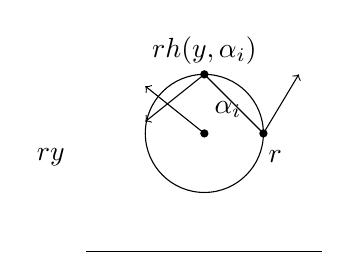
\begin{tikzpicture}[scale=1.5]
        % Drawing the vertices
        \coordinate (A) at (0,0);
        \coordinate (B) at (2,0);
        \coordinate (C) at (1.5,1);
        \coordinate (D) at (1,1.5);
        
        % Drawing the lines
        \draw (A) -- (B);
        \draw (C) -- (D);
        
        % Drawing the circle
        \draw (1, 1) circle (0.5);
        
        % Labels
        \node at (1, 1.7) {$rh(y,\alpha_i)$};
        \node at (-0.3, 0.8) {$ry$};
        \node at (1.6, 0.8) {$r$};
        \node at (1.2, 1.2) {$\alpha_i$};
        
        % Dots for the intersection points
        \fill (1, 1) circle (1pt);
        \fill (1.5, 1) circle (1pt);
        \fill (1, 1.5) circle (1pt);
        
        % Annotations
        \draw[->] (1, 1) -- (0.5, 1.4);
        \draw[->] (1.5, 1) -- (1.8, 1.5);
        \draw[->] (1, 1.5) -- (0.5, 1.1);
    \end{tikzpicture}
    \caption{Illustration of the region cut off by a tangent line to a circle with radius $r$ at a vertex of a polygon with angle $\alpha_i < \pi/2$.}
    \label{fig:small-alpha}
\end{figure}

\end{document}